\documentclass[12pt,a4paper]{article}
\usepackage{cmap} % Makes the PDF copiable. See http://tex.stackexchange.com/a/64198/25761
\usepackage[T1]{fontenc}
\usepackage[brazil]{babel}
\usepackage[utf8]{inputenc}
\usepackage{amsmath}
\usepackage{amsfonts}
\usepackage{amssymb}
\usepackage{amsthm}
\usepackage{textcomp} % \degree
\usepackage{gensymb} % \degree
\usepackage[usenames,svgnames,dvipsnames]{xcolor}
\usepackage{hyperref}
\usepackage{multicol}
\usepackage{graphicx}
\usepackage[margin=2cm]{geometry}
\usepackage{systeme}

\hypersetup{
    colorlinks = true,
    allcolors = {blue}
}

% TODO: Consider using exsheets
% http://linorg.usp.br/CTAN/macros/latex/contrib/exsheets/exsheets_en.pdf
%
% http://ctan.org/tex-archive/macros/latex/contrib/exercise/
% Options: answerdelayed,lastexercise,noanswer
\usepackage[answerdelayed,lastexercise]{exercise}

\addto\captionsbrazil{%
\def\listexercisename{Lista de exerc\'icios}%
\def\ExerciseName{Exerc\'icio}%
\def\AnswerName{Solu\c{c}\~ao do exerc\'icio}%
\def\ExerciseListName{Ex.}%
\def\AnswerListName{Solu\c{c}\~ao}%
\def\ExePartName{Parte}%
\def\ArticleOf{de\ }%
}

\renewcommand{\ExerciseHeaderTitle}{(\ExerciseTitle)\ }
\renewcommand{\ExerciseListHeader}{%\ExerciseHeaderDifficulty%
\textbf{%\ExerciseListName\
\ExerciseHeaderNB.\ %
%\ --- \
\ExerciseHeaderTitle}%
%\ExerciseHeaderOrigin
\ignorespaces}
\renewcommand{\AnswerListHeader}{\textbf{\ExerciseHeaderNB.\ (\AnswerListName)\ }}

\newcommand*\ger[1]{\operatorname{ger}\left\{#1\right\}}
\newcommand*\R{\mathbb{R}}

% Loop Space / CC BY-SA-3.0 / https://tex.stackexchange.com/a/2238/25761
\newenvironment{amatrix}[1]{%
  \left[\begin{array}{@{}*{#1}{c}|c@{}}
}{%
  \end{array}\right]
}

% Loop Space / CC BY-SA-3.0 / https://tex.stackexchange.com/a/3164/25761
%--------grstep
% For denoting a Gauss' reduction step.
% Use as: \grstep{\rho_1+\rho_3} or \grstep[2\rho_5 \\ 3\rho_6]{\rho_1+\rho_3}
\newcommand{\grstep}[2][\relax]{%
   \ensuremath{\mathrel{
       {\mathop{\longrightarrow}\limits^{#2\mathstrut}_{
                                     \begin{subarray}{l} #1 \end{subarray}}}}}}

\renewcommand{\theenumi}{\alph{enumi}}
\renewcommand\labelenumi{(\theenumi) }

\newcommand*\tipo{Prova III}
\newcommand*\turma{PRO112-02U}
\newcommand*\disciplina{ALI0001}
\newcommand*\eu{Helder G. G. de Lima}
\newcommand*\data{09/06/2018}

\author{\eu}
\title{\tipo - \disciplina}
\date{\data}

\begin{document}
\thispagestyle{empty}
\newgeometry{margin=2cm,bottom=0.5cm}
\begin{center}

\includegraphics[width=9.0cm]{marca} \\
\textbf{\tipo\ (\disciplina / \turma)} \\
Prof. \eu\footnote{
Este é um material de acesso livre distribuído sob os termos da licença \href{https://creativecommons.org/licenses/by-sa/4.0/deed.pt_BR}{Creative Commons BY-SA 4.0}}
\end{center}

\noindent Nome do(a) aluno(a): \underline{\hspace{9,7cm}} Data: \underline{\data}

%\section*{Instruções}
\begin{center}\fbox{
\begin{minipage}{14cm}

{\footnotesize
\begin{itemize}
\renewcommand{\theenumi}{\Roman{enumi}}
\item Identifique-se em todas as folhas.
\item Mantenha o celular e os demais equipamentos eletrônicos desligados durante a prova.
\item Resolva (integralmente) apenas os itens de que precisar para somar 10,0 pontos.
\end{itemize}
}

\end{minipage}
}
\end{center}

\section*{Questões}
\begin{ExerciseList}
\Exercise[title={2,0}] Considere as bases
$\alpha = \left\{ (1,3), (3,1)\right\}$
e
$\beta = \{ (2,2), (-1,1) \}$ de $\R^2$ e sejam $v, w \in \R^2$. Utilize matrizes de mudança de base para:
\begin{enumerate}
\item Calcular $[v]_{\beta}$, sabendo que
$[v]_{\alpha} =
\begin{bmatrix}
0\\2
\end{bmatrix}$.
\item Calcular $[w]_{\alpha}$, sabendo que
$[w]_{\beta} =
\begin{bmatrix}
-1\\1
\end{bmatrix}$.
\end{enumerate}
\Answer Considerando que $\beta = \{ (2,2), (-1,1) \}$ é base de $\R^2$, cada um dos vetores de $\alpha = \left\{ (1,3), (3,1)\right\}$ pode ser escrito como combinação linear dos vetores de $\beta$. Especificamente, tem-se:
\[
(1,3) = 1\cdot(2,2)+1\cdot(-1,1)\quad \text{ e }\quad
(3,1) = 1\cdot(2,2)+(-1)\cdot(-1,1)
\]
Assim,
$[ (1,3) ]_{\beta} =
\begin{bmatrix}
1 \\
1
\end{bmatrix}$,
$[ (3,1) ]_{\beta} =
\begin{bmatrix}
1 \\
-1
\end{bmatrix}$
e consequentemente
$[I]_{\beta}^{\alpha}
=
\begin{bmatrix}
1 & 1 \\
1 & -1
\end{bmatrix}$.

\begin{enumerate}
\item Pela discussão anterior, tem-se:
\[
[v]_{\beta}
= [I]_{\beta}^{\alpha} [v]_{\alpha}
= 
\begin{bmatrix}
1 & 1 \\
1 & -1
\end{bmatrix}
\cdot
\begin{bmatrix}
0\\2
\end{bmatrix}
=
\begin{bmatrix}
2\\-2
\end{bmatrix}.
\]
\item Considerando que $[I]_{\alpha}^{\beta} = ([I]_{\beta}^{\alpha})^{-1}$, tem-se:
\[
[w]_{\alpha}
= ([I]_{\beta}^{\alpha})^{-1} [w]_{\beta}
=\frac{1}{2}
\begin{bmatrix}
1 & 1 \\
1 & -1
\end{bmatrix}
\cdot
\begin{bmatrix}
-1\\1
\end{bmatrix}
=
\begin{bmatrix}
0\\-1
\end{bmatrix}.
\]
\end{enumerate}



\Exercise[title={2,0}] Dê um exemplo de uma função $f: \R^{2\times 2} \to \R$ que seja uma transformação linear e de uma $g: \R^{2\times 2} \to \R$ que não seja linear. Demonstre que suas respostas estão corretas.
\Answer Dois exemplos bem conhecidos são as funções traço e determinante. Se $A = (a_{ij})$ e $B = (b_{ij})$, então:
\begin{enumerate}
\item $f: \R^{2 \times 2} \to \R$ é definida por $f(A) = a_{11} + a_{22}$. Esta função é linear pois
\begin{align*}
  f(\alpha A + \beta B)
& = f
\left(
\alpha \begin{pmatrix}
a_{11} & a_{12} \\ a_{21} & a_{22}
\end{pmatrix}
+\beta
\begin{pmatrix}
b_{11} & b_{12} \\ b_{21} & b_{22}
\end{pmatrix}
\right)
=
f
 \begin{pmatrix}
  \alpha a_{11}+\beta b_{11}
& \alpha a_{12}+\beta b_{12}
\\\alpha a_{21}+\beta b_{21}
& \alpha a_{22}+\beta b_{22}
\end{pmatrix} \\
& = 
(\alpha a_{11}+\beta b_{11}) + (\alpha a_{22}+\beta b_{22})
= \alpha (a_{11}+a_{22}) + \beta (b_{11}+b_{22}) \\
& = \alpha f(A) + \beta f(B).
\end{align*}
\item $\operatorname{det}: \R^{2 \times 2} \to \R$, $\operatorname{det}(A) = a_{11}a_{22} - a_{21}a_{12}$ não é linear pois, por exemplo, se $A = \begin{bmatrix}
1 & 0\\0 &1
\end{bmatrix}$, então
$\operatorname{det}(2 A) = 4 \neq 2 = 2\operatorname{det}(A)$.
\end{enumerate}

\Exercise[title={2,0}] Verifique se há algum operador linear $T:\R^2 \to \R^2$ que transforma a figura $S$ na figura $S'$ conforme mostrado a seguir. Em caso afirmativo, obtenha $T(x,y)$. Justifique sua resposta.
\begin{center}
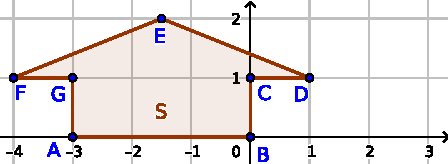
\includegraphics[width=7.0cm]{img/prova-3-pro-plano-1.pdf}
\hspace{1cm}
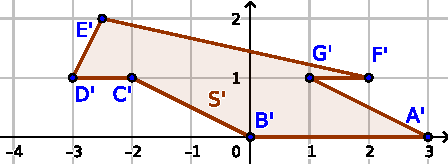
\includegraphics[width=7.0cm]{img/prova-3-pro-plano-2.pdf}
\end{center}
\Answer Sabe-se que se $\alpha = \{ v_1, v_2 \}$ é uma base de $\R^2$ e $w_1$ e $w_2$ são vetores arbitrários de $\R^2$, então a função $T: \R^2 \to \R^2$ definida por $T(c_1 v_1 + c_2 v_2) = c_1 w_1 + c_2 w_2$ é uma (a única) transformação linear que leva $v_1$ em $w_1$ e $v_2$ em $w_2$. Assim, como $\alpha = \{ A, C \} = \{ (-3,0), (0,1) \}$ é uma base de $\R^2$ (por quê?), pode-se dizer que existe uma única transformação linear $T$ que leva $A = (-3,0)$ em $A^\prime = (3,0)$ e $C=(0,1)$ em $C^\prime = (-2,1)$. Tal transformação linear é dada por
\begin{align*}
T(x,y)
& = T\left( \frac{-x}{3}(-3,0) + y(0,1) \right)
  = \frac{-x}{3} T(-3,0) + yT(0,1)\\
& = \frac{-x}{3} (3,0) + y(-2,1)
  = (-x-2y,y).
\end{align*}
Uma verificação direta mostra que este operador linear leva cada um dos demais pontos indicados na primeira figura nos pontos correspondentes da segunda figura.

\Exercise[title={2,0}] Se $S$ é o espaço das matrizes simétricas de ordem $2 \times 2$ e $T: S \to \R^3$ é definida por
\[
T\begin{pmatrix}
x & y\\y&z
\end{pmatrix} = (x,3z, x-3z), \quad \forall x, y,z \in \R
\]
determine se $T$ é um isomorfismo. Justifique sua resposta.
\Answer Como $T\begin{pmatrix}
0 & 1 \\ 1 & 0
\end{pmatrix} = (0, 0, 0)$, tem-se $N(T) \neq \left\{ \begin{pmatrix}
0 & 0 \\ 0 & 0
\end{pmatrix} \right\}$, e deste modo $T$ não é injetora. Com isso, $T$ também não é considerada um isomorfismo.

\textbf{Solução alternativa}: Para que $T$ fosse um isomorfismo, seria preciso que $T$ fosse, em particular, sobrejetora. Para que isso ocorresse, todo vetor de $\R^3$ deveria pertencer à imagem de $T$. No entanto, $w = (0,0,1) \in \R^3$ e $w \not\in \operatorname{Im}(T)$, pois para isso seria preciso que $(0,0,1) = (x,3z,x-3z)$, para algum $x \in \R$ e algum $z \in \R$. Isso implicaria que $x = 0 = z$ ao mesmo tempo em que $x-3z = 1$, o que é impossível. Assim, $T$ não é um isomorfismo.

\Exercise[title={2,0}] Seja $L: P_1 \to \R^2$ definida por $L(q) = (q(-1), q(1))$, para todo $q(x) = ax+b \in P_1$.
\begin{enumerate}
\item Obtenha a matriz de $L$ em relação às bases $\alpha = \{1, x\}$ de $P_1$ e $\beta = \{(1,0),(0,1)\}$ de $\R^2$.
\item Obtenha, se existir, a transformação inversa, $L^{-1}(c,d)$ e calcule o polinômio $L^{-1}(2,3)$.
\end{enumerate}
\Answer Conforme a definição da transformação $L$, para todo $q(x) = ax+b \in P_1$ tem-se: $L(q) = L(ax+b) = (a(-1)+b, a(1)+b) = (-a+b,a+b)$.
\begin{enumerate}
\item Ao aplicar $L$ nos vetores da base $\alpha$, obtém-se $L(1)=(1,1)$ e $L(x)=(-1,1)$. Então a matriz de $L$ em relação às bases $\alpha$ e $\beta$ é $[L]_\beta^\alpha =
\begin{bmatrix}
1 & -1 \\ 1 & 1
\end{bmatrix}$.
\item A inversa de uma transformação linear $L$ pode ser determinada a partir de sua matriz $[L^{-1}]_\alpha^\beta$, que é a inversa da matriz $[L]_\beta^\alpha$ da transformação $L$, isto é,
\[
[L^{-1}]_\alpha^\beta
= ([L]_\beta^\alpha)^{-1}
= \begin{bmatrix}
1 & -1 \\ 1 & 1
\end{bmatrix}^{-1}
= \begin{bmatrix}
1/2 & 1/2 \\ -1/2 & 1/2
\end{bmatrix}.
\]
Assim,
\[
[L^{-1}(c,d)]_{\alpha}
= [L^{-1}]_\alpha^\beta
[(c,d)]_{\beta}
=
\begin{bmatrix}
1/2 & 1/2 \\ -1/2 & 1/2
\end{bmatrix}
\begin{bmatrix}
c\\d
\end{bmatrix}
=
\begin{bmatrix}
\frac{c+d}{2}\\\frac{-c+d}{2}
\end{bmatrix},
\]
o que significa que $L^{-1}(c,d) = \left(\frac{c+d}{2}\right)
+\left(\frac{-c+d}{2}\right)x$ e $L^{-1}(2,3) = \frac{5}{2} + \frac{1}{2}x$.
\end{enumerate}

\Exercise[title={2,0}] Prove ou dê um contra-exemplo:
\begin{enumerate}
\item Toda transformação linear $T: \R^2 \to \R^3$ é sobrejetora
\item Nenhum operador linear \textbf{injetor} $T: \R^2 \to \R^2$ satisfaz $T(1,5)=(6,6)$ e $T(5,1) = (3,3)$.
\end{enumerate}
\Answer
\begin{enumerate}
\item \textbf{Falso}. A transformação linear nula, dada por $T(x,y) = (0,0,0)$ não é sobrejetora. Na verdade, \textit{nenhuma} transformação linear de $\R^2$ para $\R^3$ é sobrejetora, pois neste caso teríamos:
\[
\dim(N(T)) + \dim(\R^3) = \dim(\R^2) \Rightarrow \dim(N(T)) = 2 - 3 = -1,
\]
o que não faria sentido, já que a dimensão de um espaço é sempre maior ou igual a zero.
\item Qualquer transformação linear que satisfaça $T(5,1) = (3,3)$, também deve satisfazer
\[
T(10,2) = T(2\cdot (5,1)) = 2 \cdot T(5,1) = 2\cdot (3,3) = (6,6) = T(1,5).
\]
Em outras palavras, $T$ deve levar os pontos distintos $(10,2)$ e $(1,5)$ na mesma imagem $(6,6)$, ou seja, $T$ não pode ser injetora.

\textbf{Solução alternativa}: Como $\alpha = \{ (1, 5), (5, 1) \}$ é uma base de $\R^2$, pode-se concluir que existe um único operador linear $T: \R^2 \to \R^2$ que satisfaz $T(1,5)=(6,6)$ e $T(5,1) = (3,3)$, o qual é definido por
\[
T(x,y) = \left(\frac{3}{8}x+\frac{9}{8}y,\frac{3}{8}x+\frac{9}{8}y\right), \forall (x,y) \in \R^2.
\]
Como este operador linear não é injetor (pois $N(T) = \ger{(-3,1)} \neq \{ (0,0) \}$), conclui-se que não existe um operador linear que satisfaça as condições estipuladas.
\end{enumerate}
\end{ExerciseList}

\begin{center}
BOA PROVA!
\end{center}

\newpage
\restoregeometry
\section*{Respostas}
\shipoutAnswer
\end{document}
